You pass through the barrier of fog, and enter into a curious scene.\\

Two columns of hollowed prisoners stand here in the yard, chained together at their ankles. In their hands, they bear an assortment of makeshift armaments: flagpoles, stockades, and railings filed into crude spears, and shields fashioned from hacked-apart mess tables.\\

The prisoners waver idly in their formation, adrift in their own maddened thoughts. A revolt forgotten in its infancy by both guard and revolutionary alike. Yet their heads pick up at the sound of your approaching footfalls. And the phalanx wheels in your direction, its rows of ramshackle spears dropping into a defensive posture.

\subsection*{Victory Condition}
Defeat all enemies

\subsection*{Doom Events}
For this encounter, \emph{doom events} are triggered by the remaining number of Hollowed Prisoner Phalanxes, not \emph{round tallies}.

\begin{itemize}
\item \textbf{10 Remaining:} \emph{The phalanx begins to march--lurching, and badly out of step.} Begin the encounter by rolling on table A.
\item \textbf{7 Remaining:} \emph{The Lost Phalanx drags its dead members along by their chains, severely slowing the formation.} The Lost Phalanx loses 1 Move value.
\item \textbf{4 Remaining:} \emph{The remaining hollows can no longer hold their formation.} The last 4 Hollowed Prisoner Phalanx entities are no longer part of The Lost Phalanx formation, and act as individual entities. Roll on table B for this and all future Rounds. The remaining enemies begin this Round with \emph{Shield Up!} present on their sheets.
\end{itemize}

\pagebreak

\subsection*{Encounter Tables}
\begin{tcolorbox}
\textbf{A - The Lost Phalanx}\\
\textbf{Roll:} 2D6
\begin{center}
\begin{tabular}{ L | L | L }
\multicolumn{1}{c|}{\textbf{2}} & 
\multicolumn{1}{c|}{\textbf{3}} & 
\multicolumn{1}{c}{\textbf{4-5}} \\
\emph{Charge!} &
\emph{Thrown Debris.} Move &
Move. \emph{Makeshift Spear} \\
\hline
\multicolumn{1}{c|}{\textbf{6}} & 
\multicolumn{1}{c|}{\textbf{7}} & 
\multicolumn{1}{c}{\textbf{8}} \\
\textbf{A:} \emph{Shield Push. Makeshift Spear}\newline \textbf{B:} \emph{Thrown Debris.} Move &
\textbf{A:} \emph{Shield Push. Makeshift Spear}\newline \textbf{B:} Move. \emph{Makeshift Spear} &
\textbf{A:} \emph{Shield Push. Makeshift Spear}\newline \textbf{B:} \emph{Thrown Debris.} Move \\
\hline
\multicolumn{1}{c|}{\textbf{9-10}} & 
\multicolumn{1}{c|}{\textbf{11}} & 
\multicolumn{1}{c}{\textbf{12}} \\
Move. \emph{Makeshift Spear} &
\emph{Thrown Debris.} Move &
\emph{Charge!}
\end{tabular}
\end{center}
\end{tcolorbox}
\ \\

\begin{tcolorbox}
\textbf{Note:} Look carefully. There is both \emph{Shield Push} and \emph{Shield Bash} in these tables, which are different attacks.
\end{tcolorbox}
\ \\

\begin{tcolorbox}
\textbf{Note:} Resolve the next conditional behavior if no entity in the front row is capable of resolving the first listed attack.
\end{tcolorbox}
\ \\

\begin{tcolorbox}
\textbf{B - Hollowed Prisoner Phalanxes}\\
\textbf{Roll:} 1D6
\begin{center}
\begin{tabular}{ L | L | L }
\multicolumn{1}{c|}{\textbf{1}} & 
\multicolumn{1}{c|}{\textbf{2-5}} & 
\multicolumn{1}{c}{\textbf{6}} \\

\textbf{A:} \emph{Thrown Debris}\newline \textbf{B:} Move. \emph{Shield Bash} &
\emph{Shield Up!} Move. \emph{Makeshift Spear}\newline \emph{This result is only exhausted after its third token} &
\textbf{A:} \emph{Thrown Debris}\newline \textbf{B:} Move. \emph{Shield Bash}
\end{tabular}
\end{center}
\textbf{Note:} All remaining enemies share a single roll. Resolve the remaining enemies’ Turns in any order of the player’s choosing.
\end{tcolorbox}

\pagebreak

\subsection*{Enemy Sheets}
\hrule
\ \\
{\large \textbf{The Lost Phalanx}}\\\\
\begin{tabular}{s s s}
\textbf{HP:} N/A & \multicolumn{2}{l}{\textbf{Move:} 3}\\
\end{tabular}\\

\emph{Formation Fighter:} This entity consists of multiple Hollowed Prisoner Phalanxes. All members are immune to Knockback and Knockdown. See the Formation Fighter Rules section on the next page for details.\\

\emph{Shieldwall:} All entities in this formation always possess \emph{Shield Up!} and have unlimited shield Stability.\\

\textbf{Attacks:}
\begin{itemize}
\item \emph{Charge!} - Move the ‘front’ towards the character in a straight or snaking line, until any member attempts to Move onto an impassable tile (including the character’s position). Once any member’s movement is halted, end the Move and fill-in the formation. If the character’s position is encountered during this movement, inflict 2 \emph{Unparryable} and \emph{Undodgeable} Crush damage, Knockback 2, and Knockdown on the character.\newline \emph{Always resolve this attack, regardless of whether it will strike the character.}
\end{itemize}
\hrule
\ \\
\begin{tcolorbox}
\textbf{Hint:} Because of \emph{Shieldwall}, there’s no need to track \emph{Shield Up!} or shield Stability/Durability for individual members of The Lost Phalanx. Just reduce all incoming damage by 1 for each member.
\end{tcolorbox}
\begin{tcolorbox}
\textbf{Hint:} \emph{Charge!} has \emph{Undodgeable} damage, but the character can still move out of the formation’s way via their \emph{Dodge!} if it has implicit Move
\end{tcolorbox}
\ \\
\hrule
\ \\
{\large \textbf{Hollowed Prisoner Phalanx}}\\\\
\begin{tabular}{s s s}
\textbf{HP:} 4 & \multicolumn{2}{l}{\textbf{Move:} 2 (when not in formation)}\\
\textbf{Shield Def:} 1 & \textbf{Shield Stab:} 5 & \textbf{Shield Dur:} 1\\
\end{tabular}\\

\emph{Hollow:} This entity ignores the Stunned, Charmed, Maddened, and Fear conditions.\\

\textbf{Attacks:}
\begin{itemize}
\item \emph{Makeshift Spear} - Deal 1 Pierce ranged melee damage to an entity within 2 tiles. Do not remove \emph{Shield Up!}
\item \emph{Shield Push} - Inflict \emph{Unparryable} Knockback 1 to an adjacent entity. Do not remove \emph{Shield Up!}
\item \emph{Shield Bash} - Deal 1 \emph{Unparryable} Crush damage and Knockback 1 to an adjacent entity. Do not remove \emph{Shield Up!}
\item \emph{Thrown Debris} - Deal 1 Crush ranged damage to an entity that is within 2-3 tiles.
\end{itemize}
\hrule

\begin{tcolorbox}
\textbf{Note:} If entities are not part of The Lost Phalanx formation, they no longer benefit from \emph{Shieldwall} or \emph{Formation Fighter}.
\end{tcolorbox}

\pagebreak

\subsection*{Formation Fighter Rules}
A Formation Fighter is a group of entities that all Move and act as a single unit. However, each entity still attacks individually and retains its own \textbf{HP}. Due to the large number of identical enemies, it would be easier to place damage directly on enemy tokens instead of tracking them via \textbf{HP} circles.\\

\textbf{The Formation} -- The Lost Phalanx must maintain its ‘two columns’ formation as best as possible, though it may snake and bend. See the example images below.\\

\textbf{Movement} -- Start by moving members of the ‘front’ simultaneously towards the character--up to the formation’s Move value and keeping all of its members adjacent. Then fill-in the rest of the phalanx behind the front (giving them whatever bonus Move necessary to complete the formation).\\
The ‘front’ is whichever row is closest to the character at the start of the Turn (in terms of actual movement, not raw hexes). If the character is positioned to one side of the formation, so that three rows are equidistant, then the formation Moves via its nearest column instead (i.e: sideways).\\
When a member dies, the formation will fill-in towards the front next time it commits Move. If a member of the front dies, Move the remainder as normal and fill-in a member to the front afterwards.\\
\emph{When maneuvering around obstacles, occasionally a member of the front may not be able to use their full Move value because other members need to ‘pivot’ to catch up.}

\subsection*{Movement Example Images}
\begin{center}
\framebox{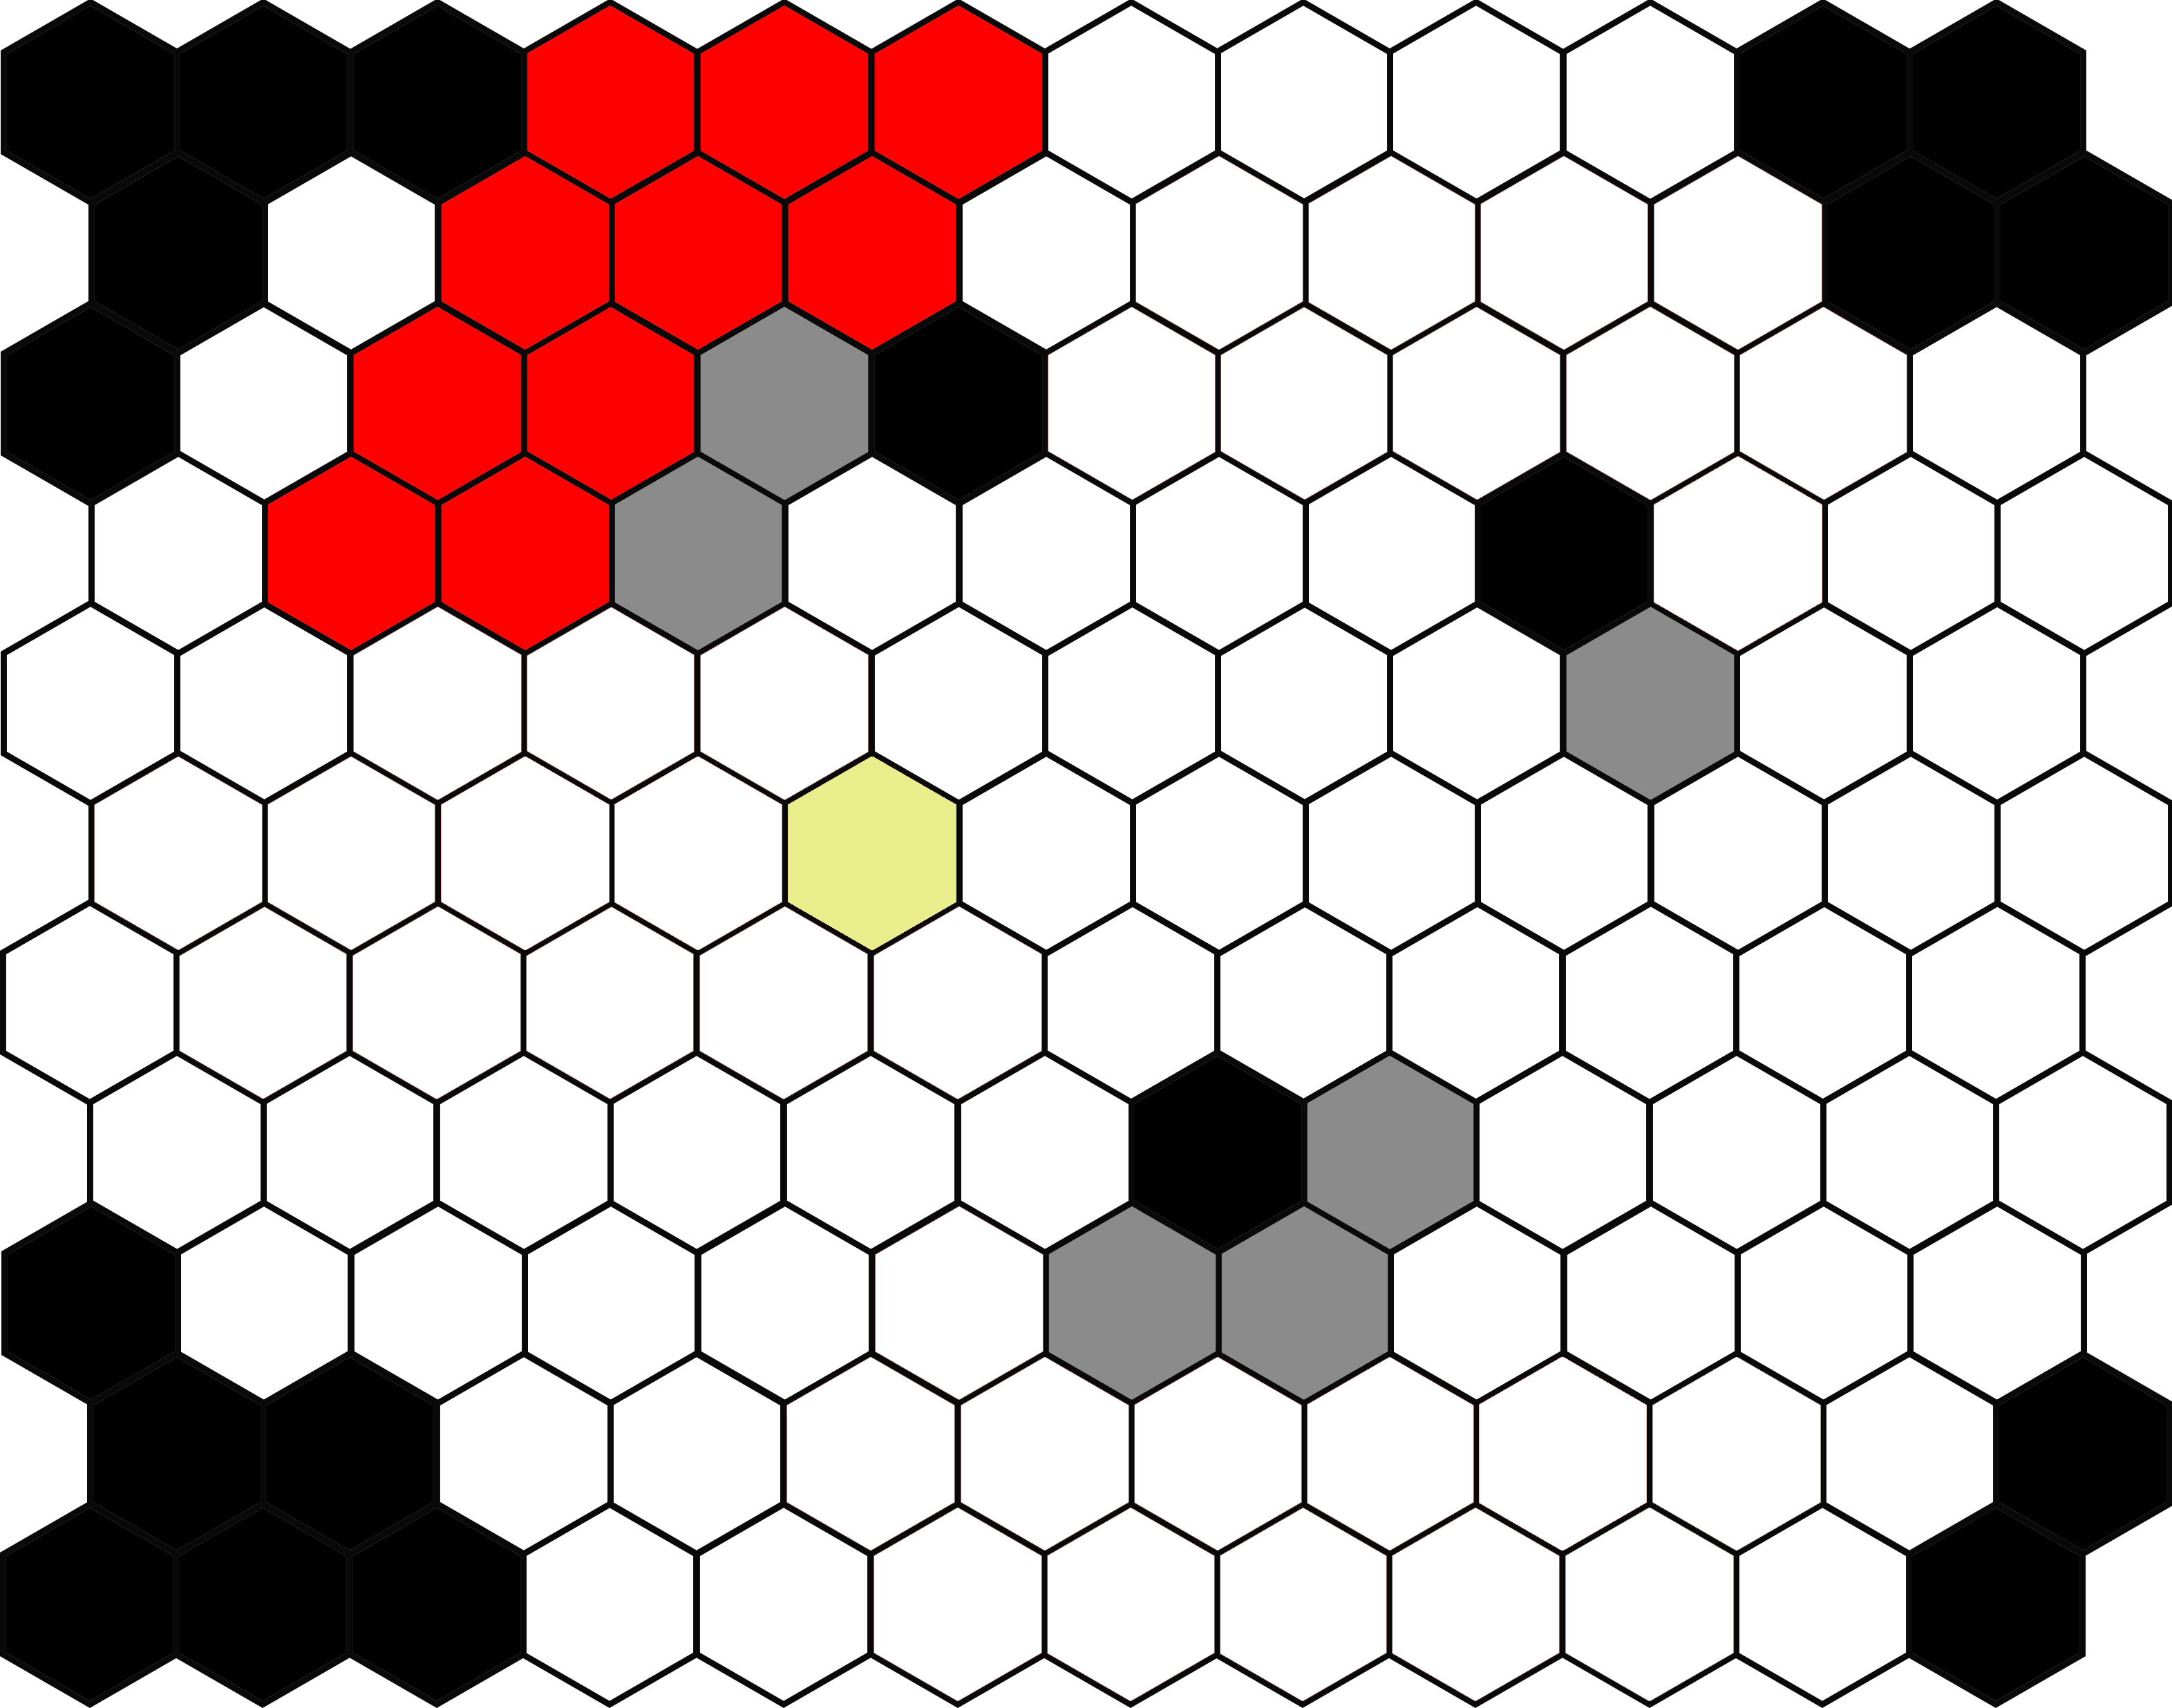
\includegraphics[width = 0.3\textwidth]{./maps/c214a.png}}
\framebox{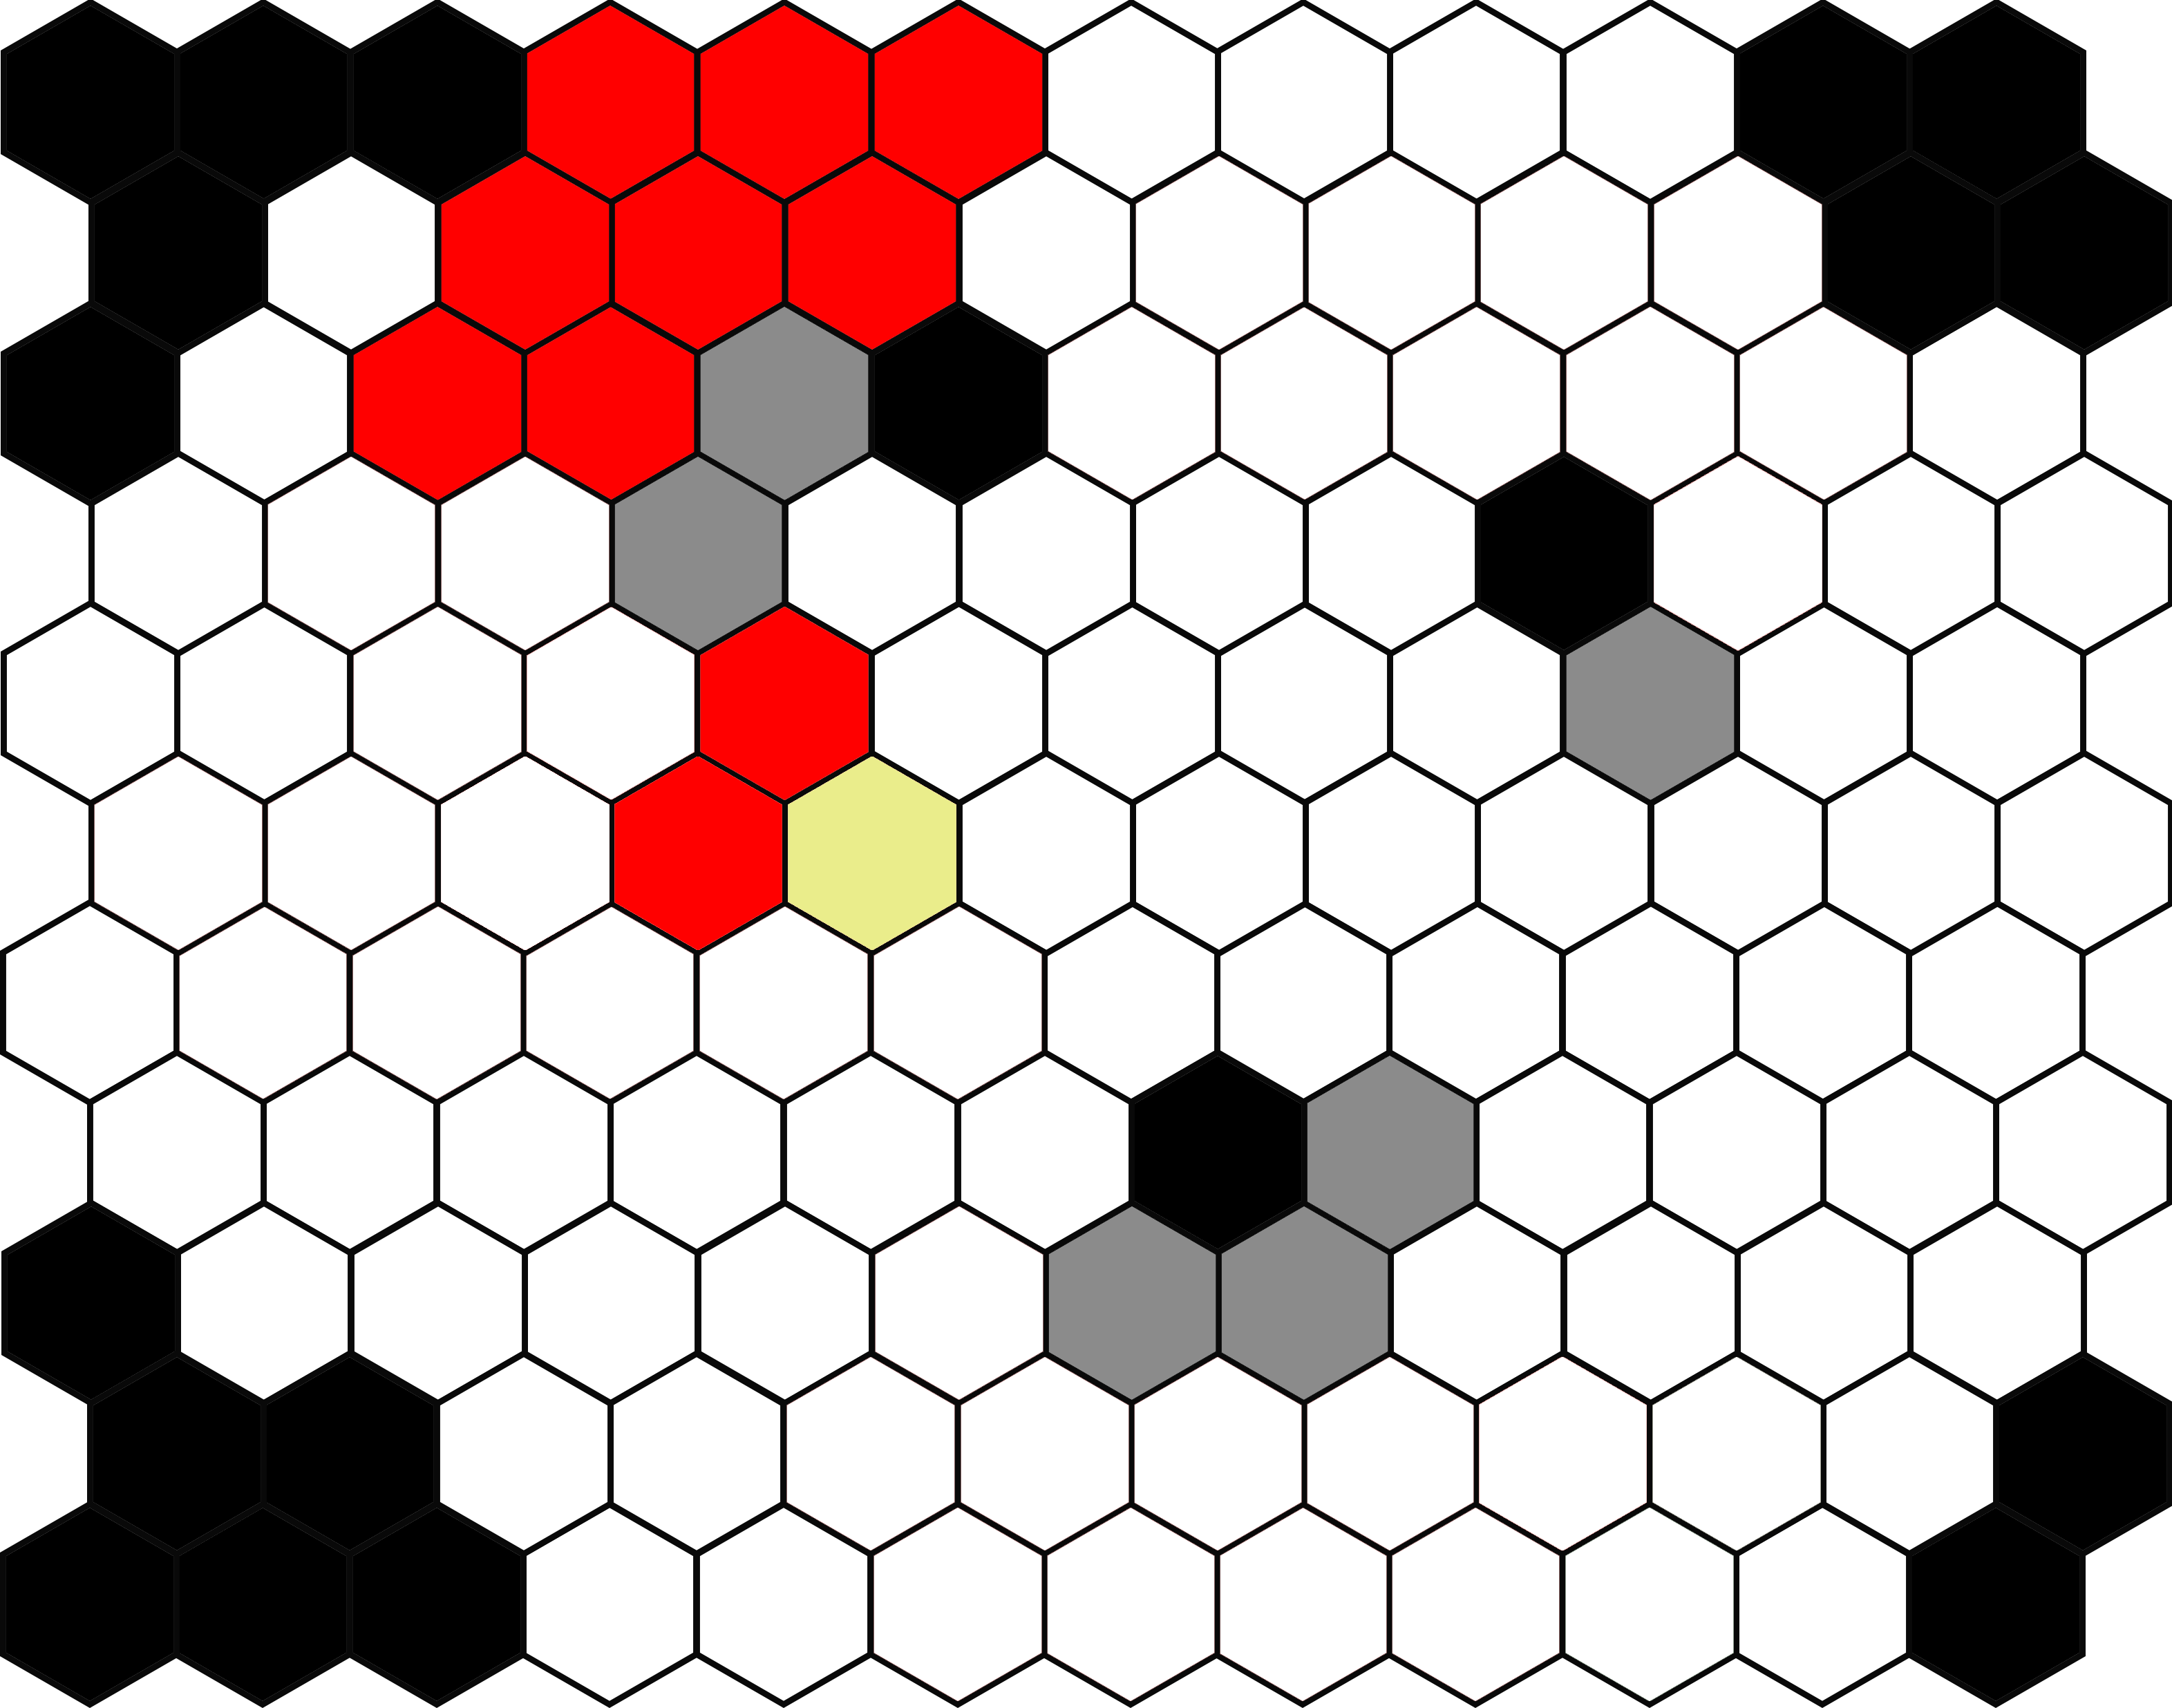
\includegraphics[width = 0.3\textwidth]{./maps/c214b.png}}
\framebox{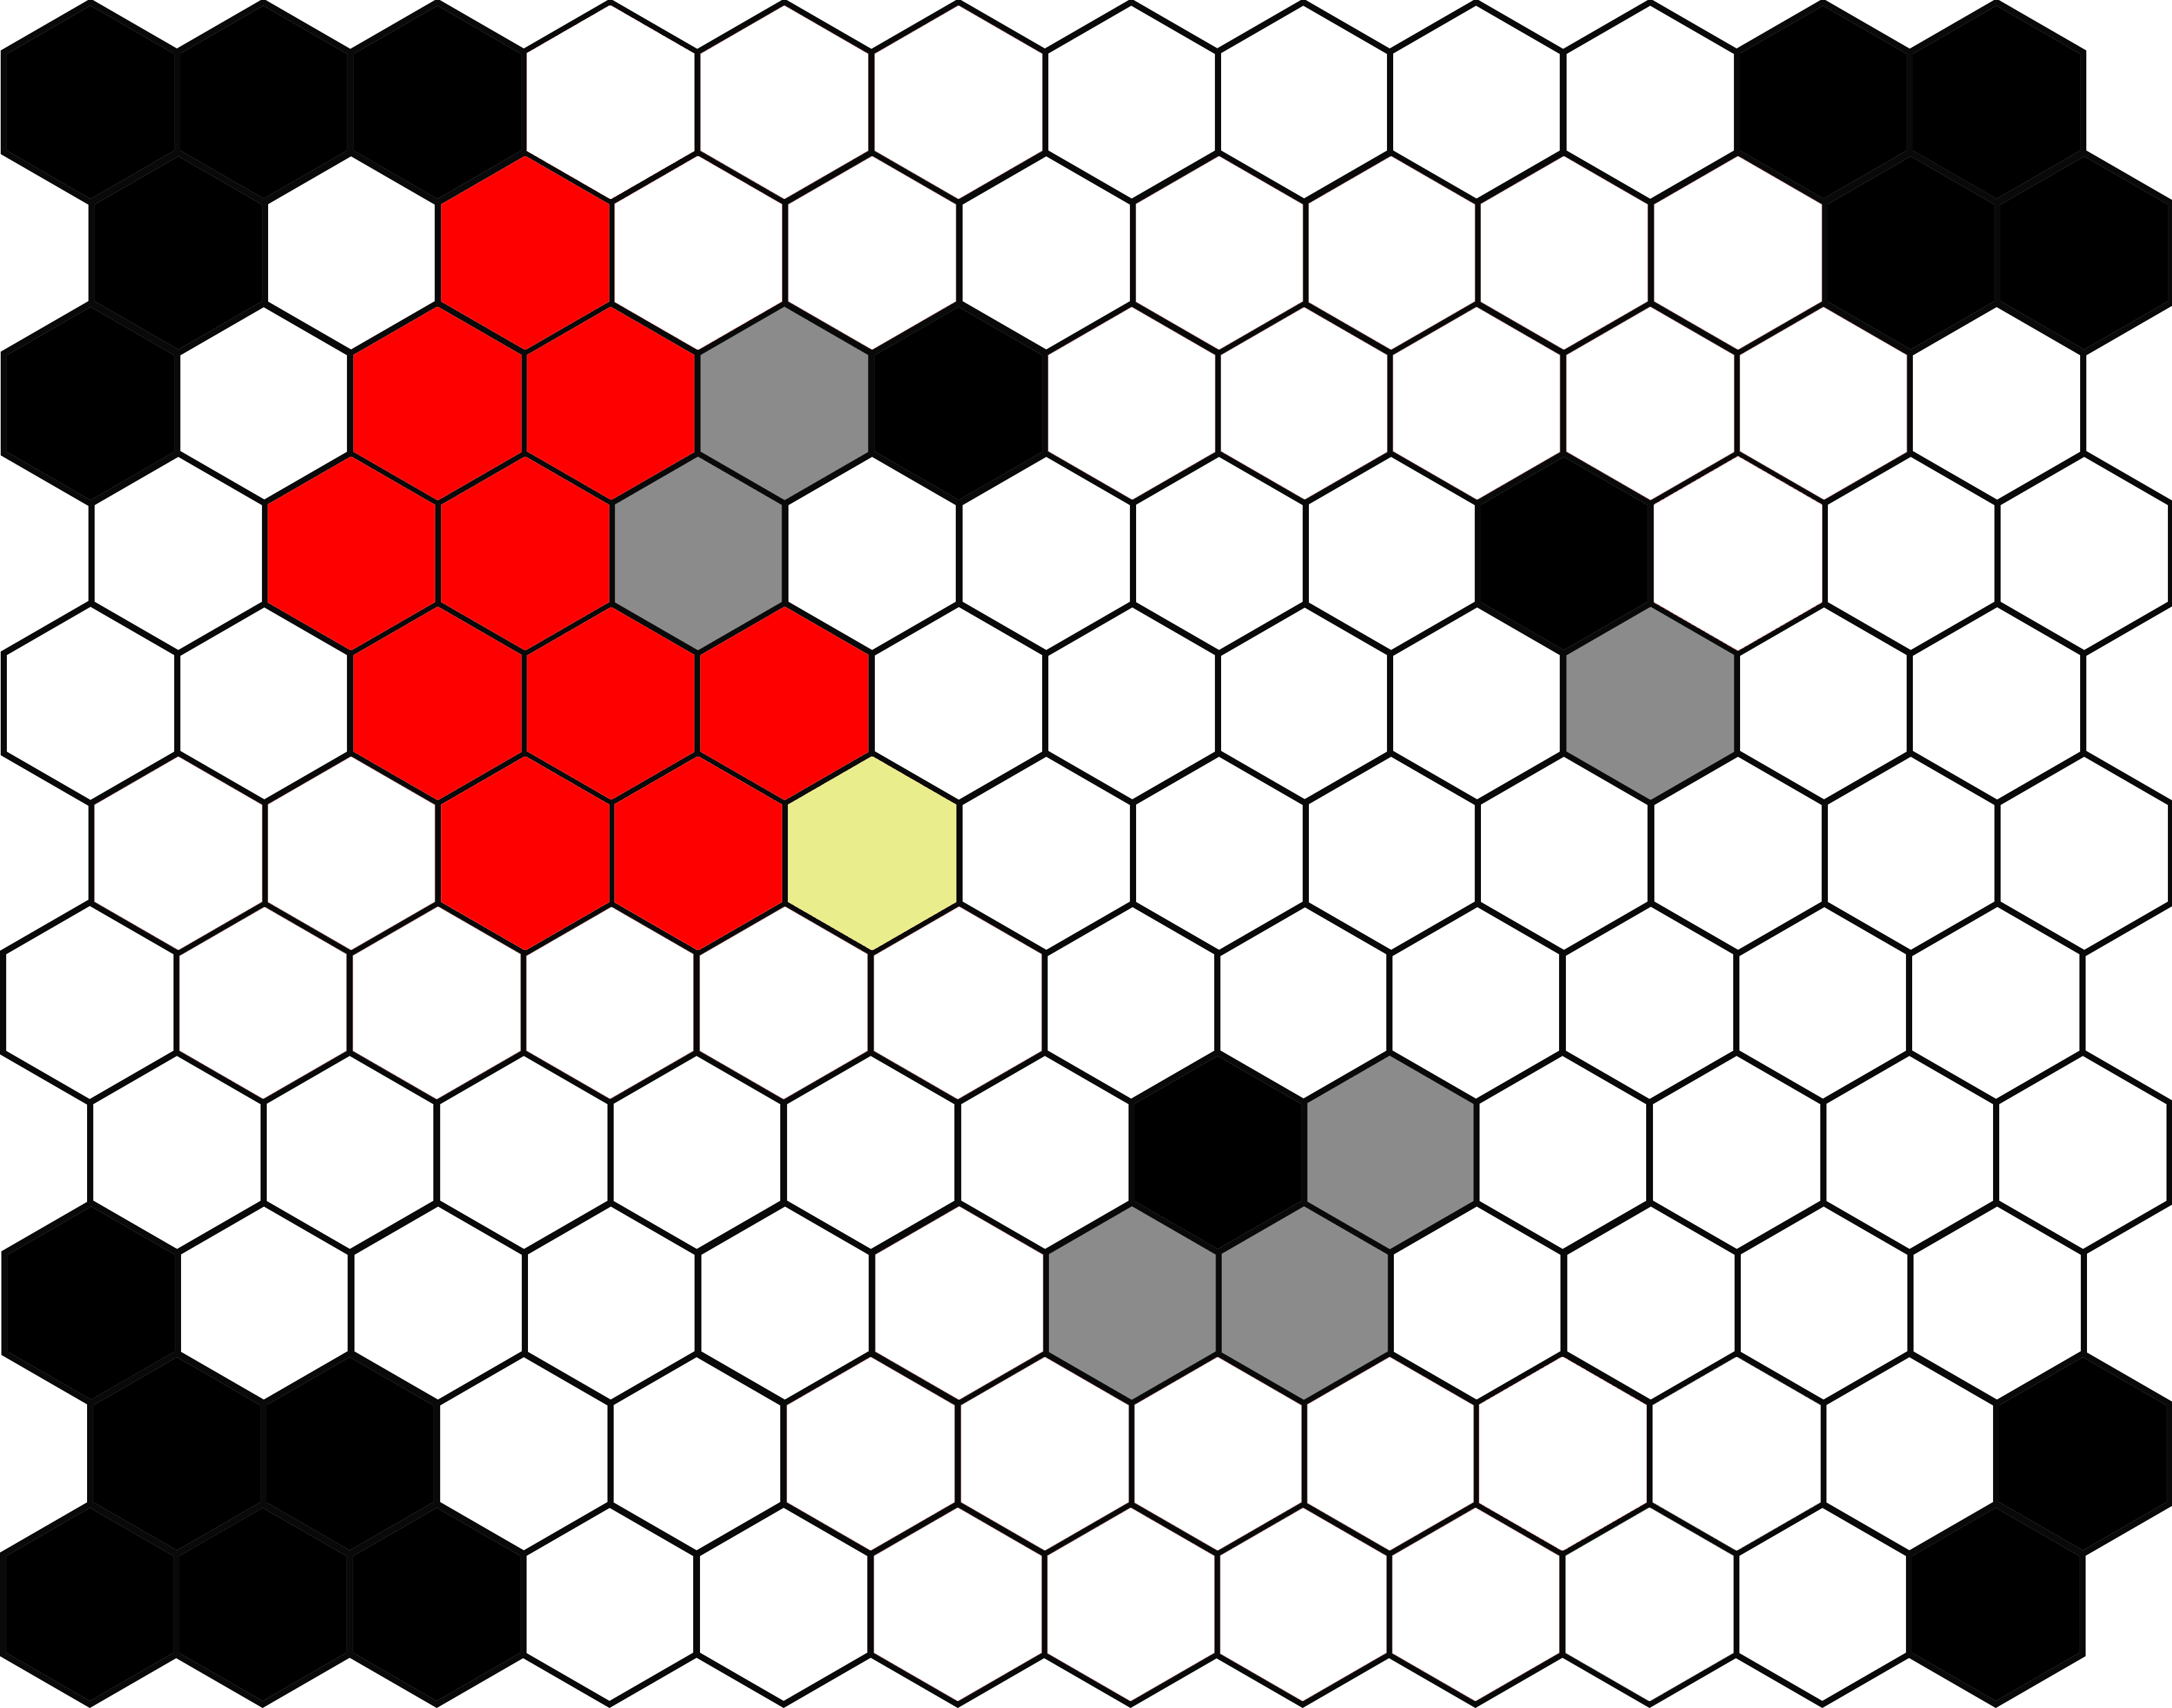
\includegraphics[width = 0.3\textwidth]{./maps/c214c.png}}
\\
\emph{From left to right:\\
(1) The formation (red) will move towards the character (goldenrod) during its Turn.\\
(2) Its Move begins with the members of the first row.\\
(3) Then the rest of the phalanx fills in, maintaining the formation as best as possible.}\\

\framebox{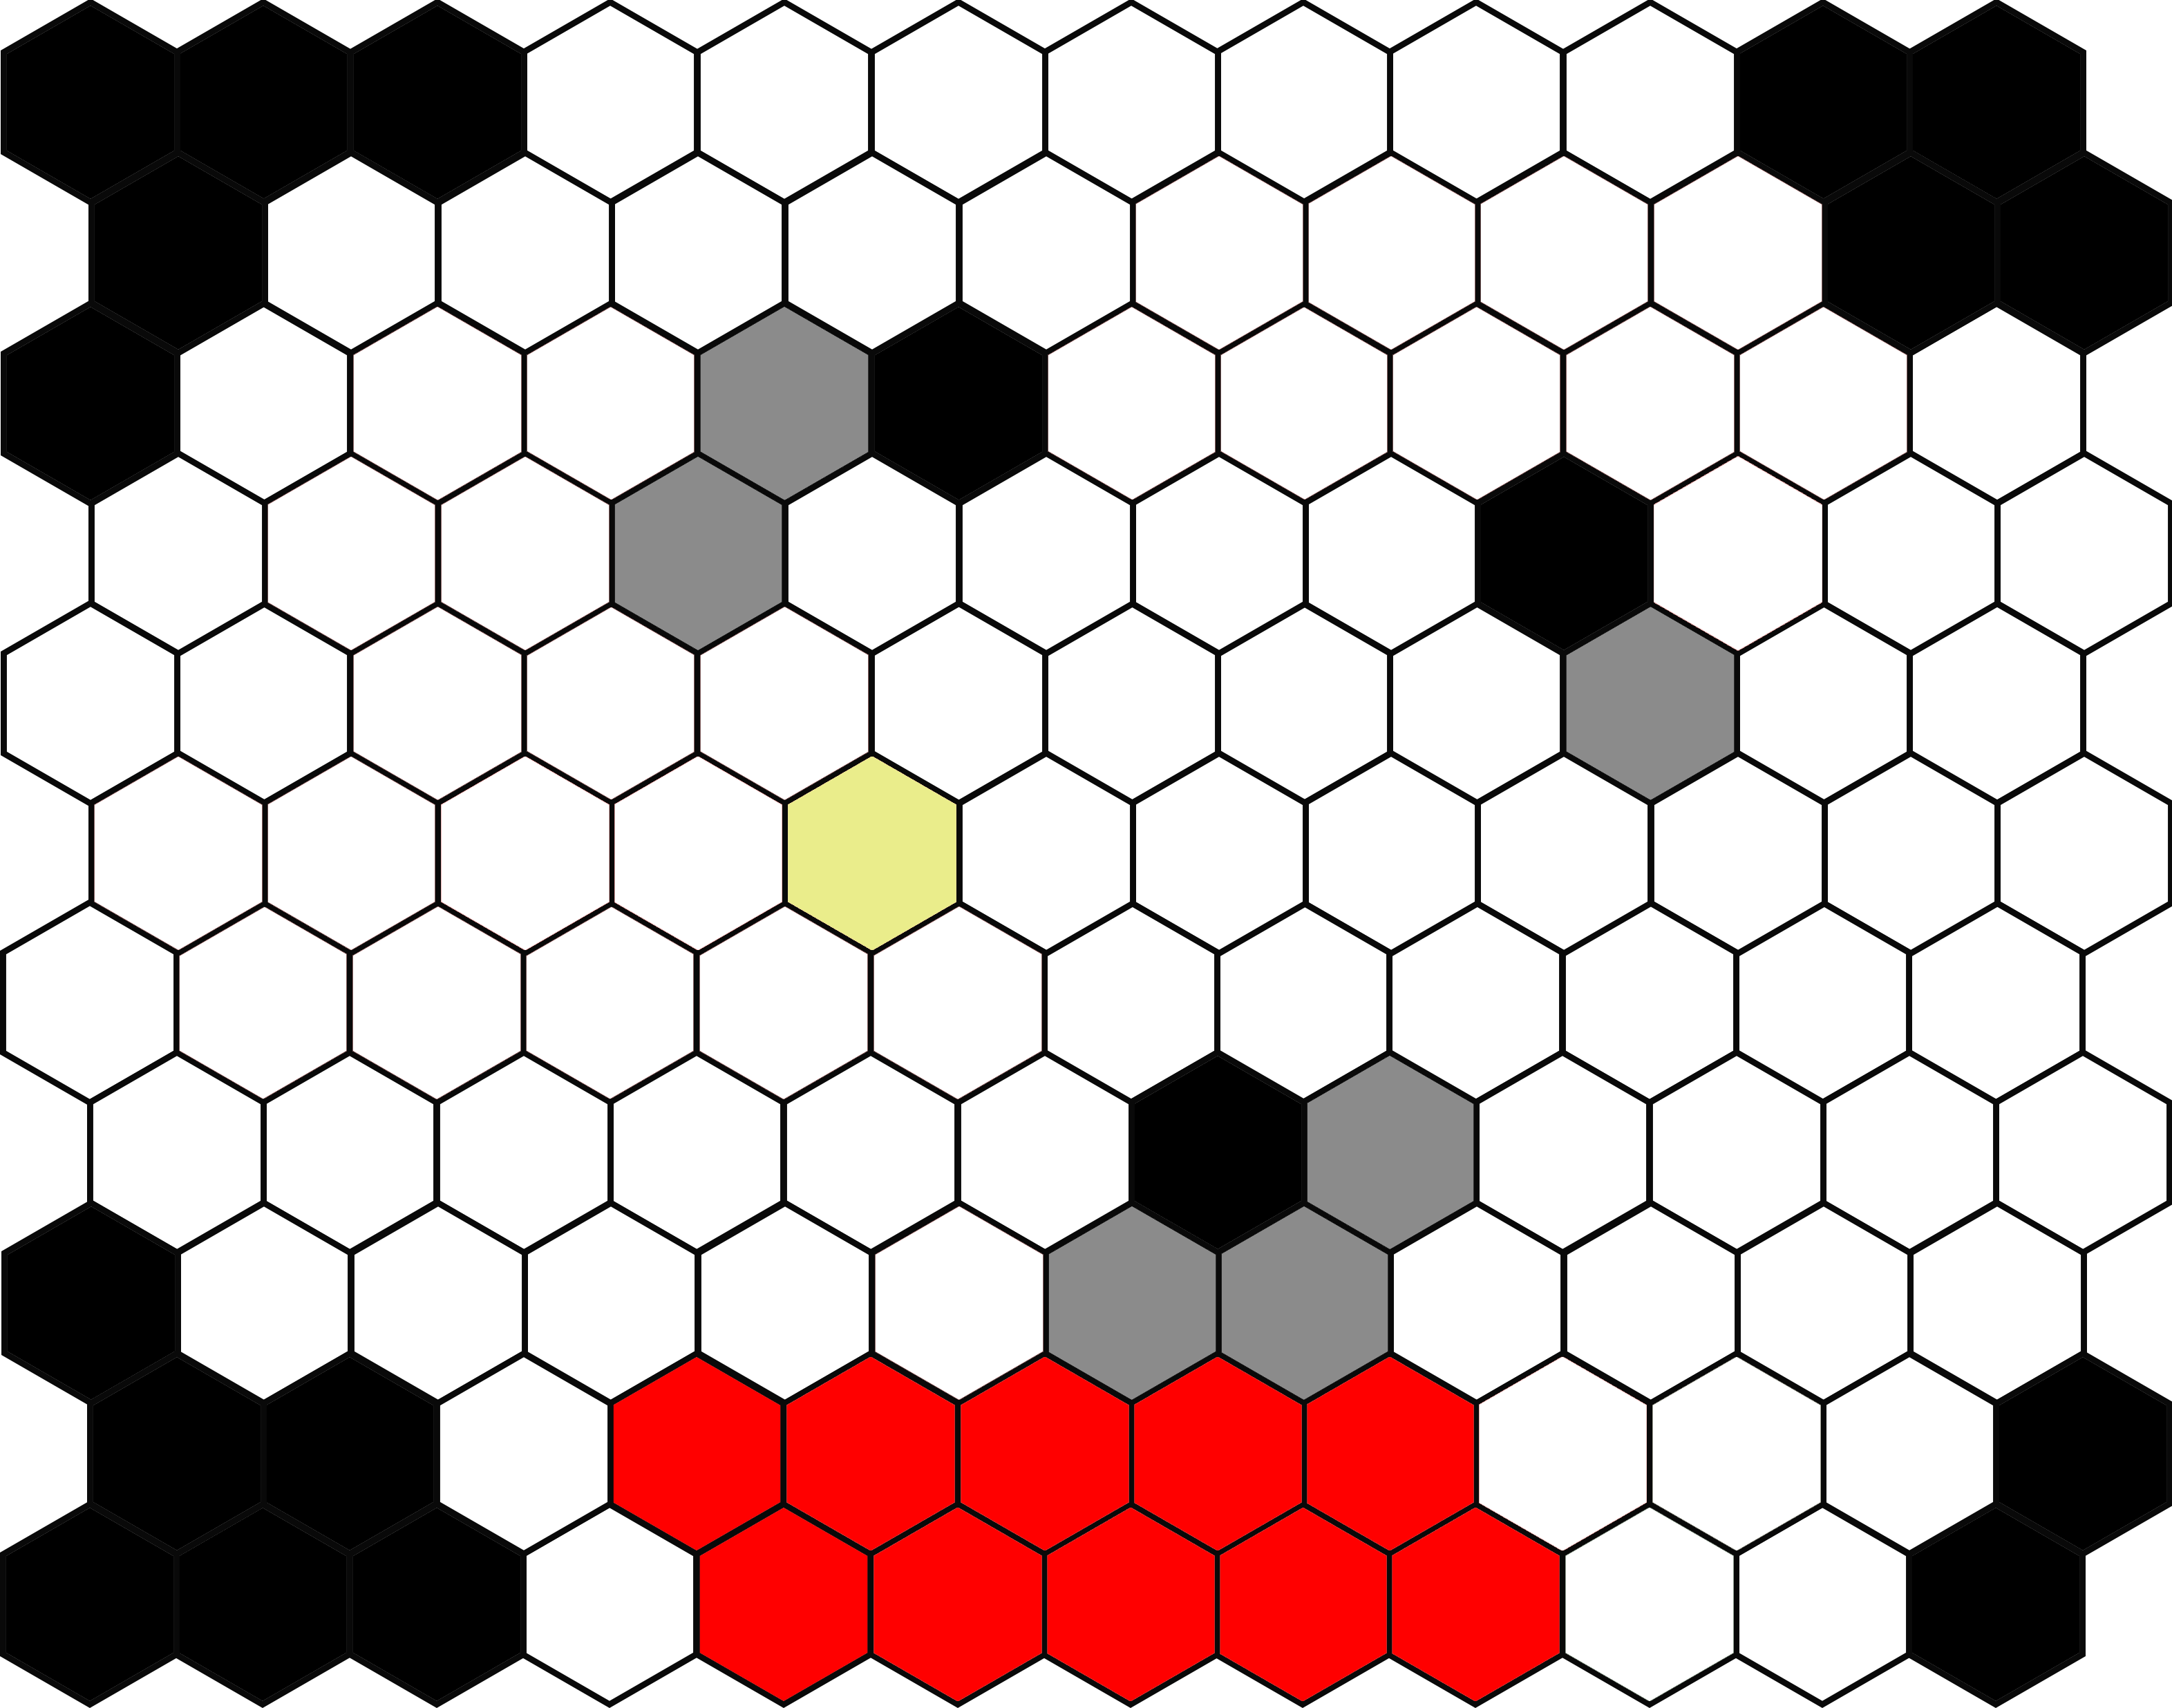
\includegraphics[width = 0.3\textwidth]{./maps/c214d.png}}
\framebox{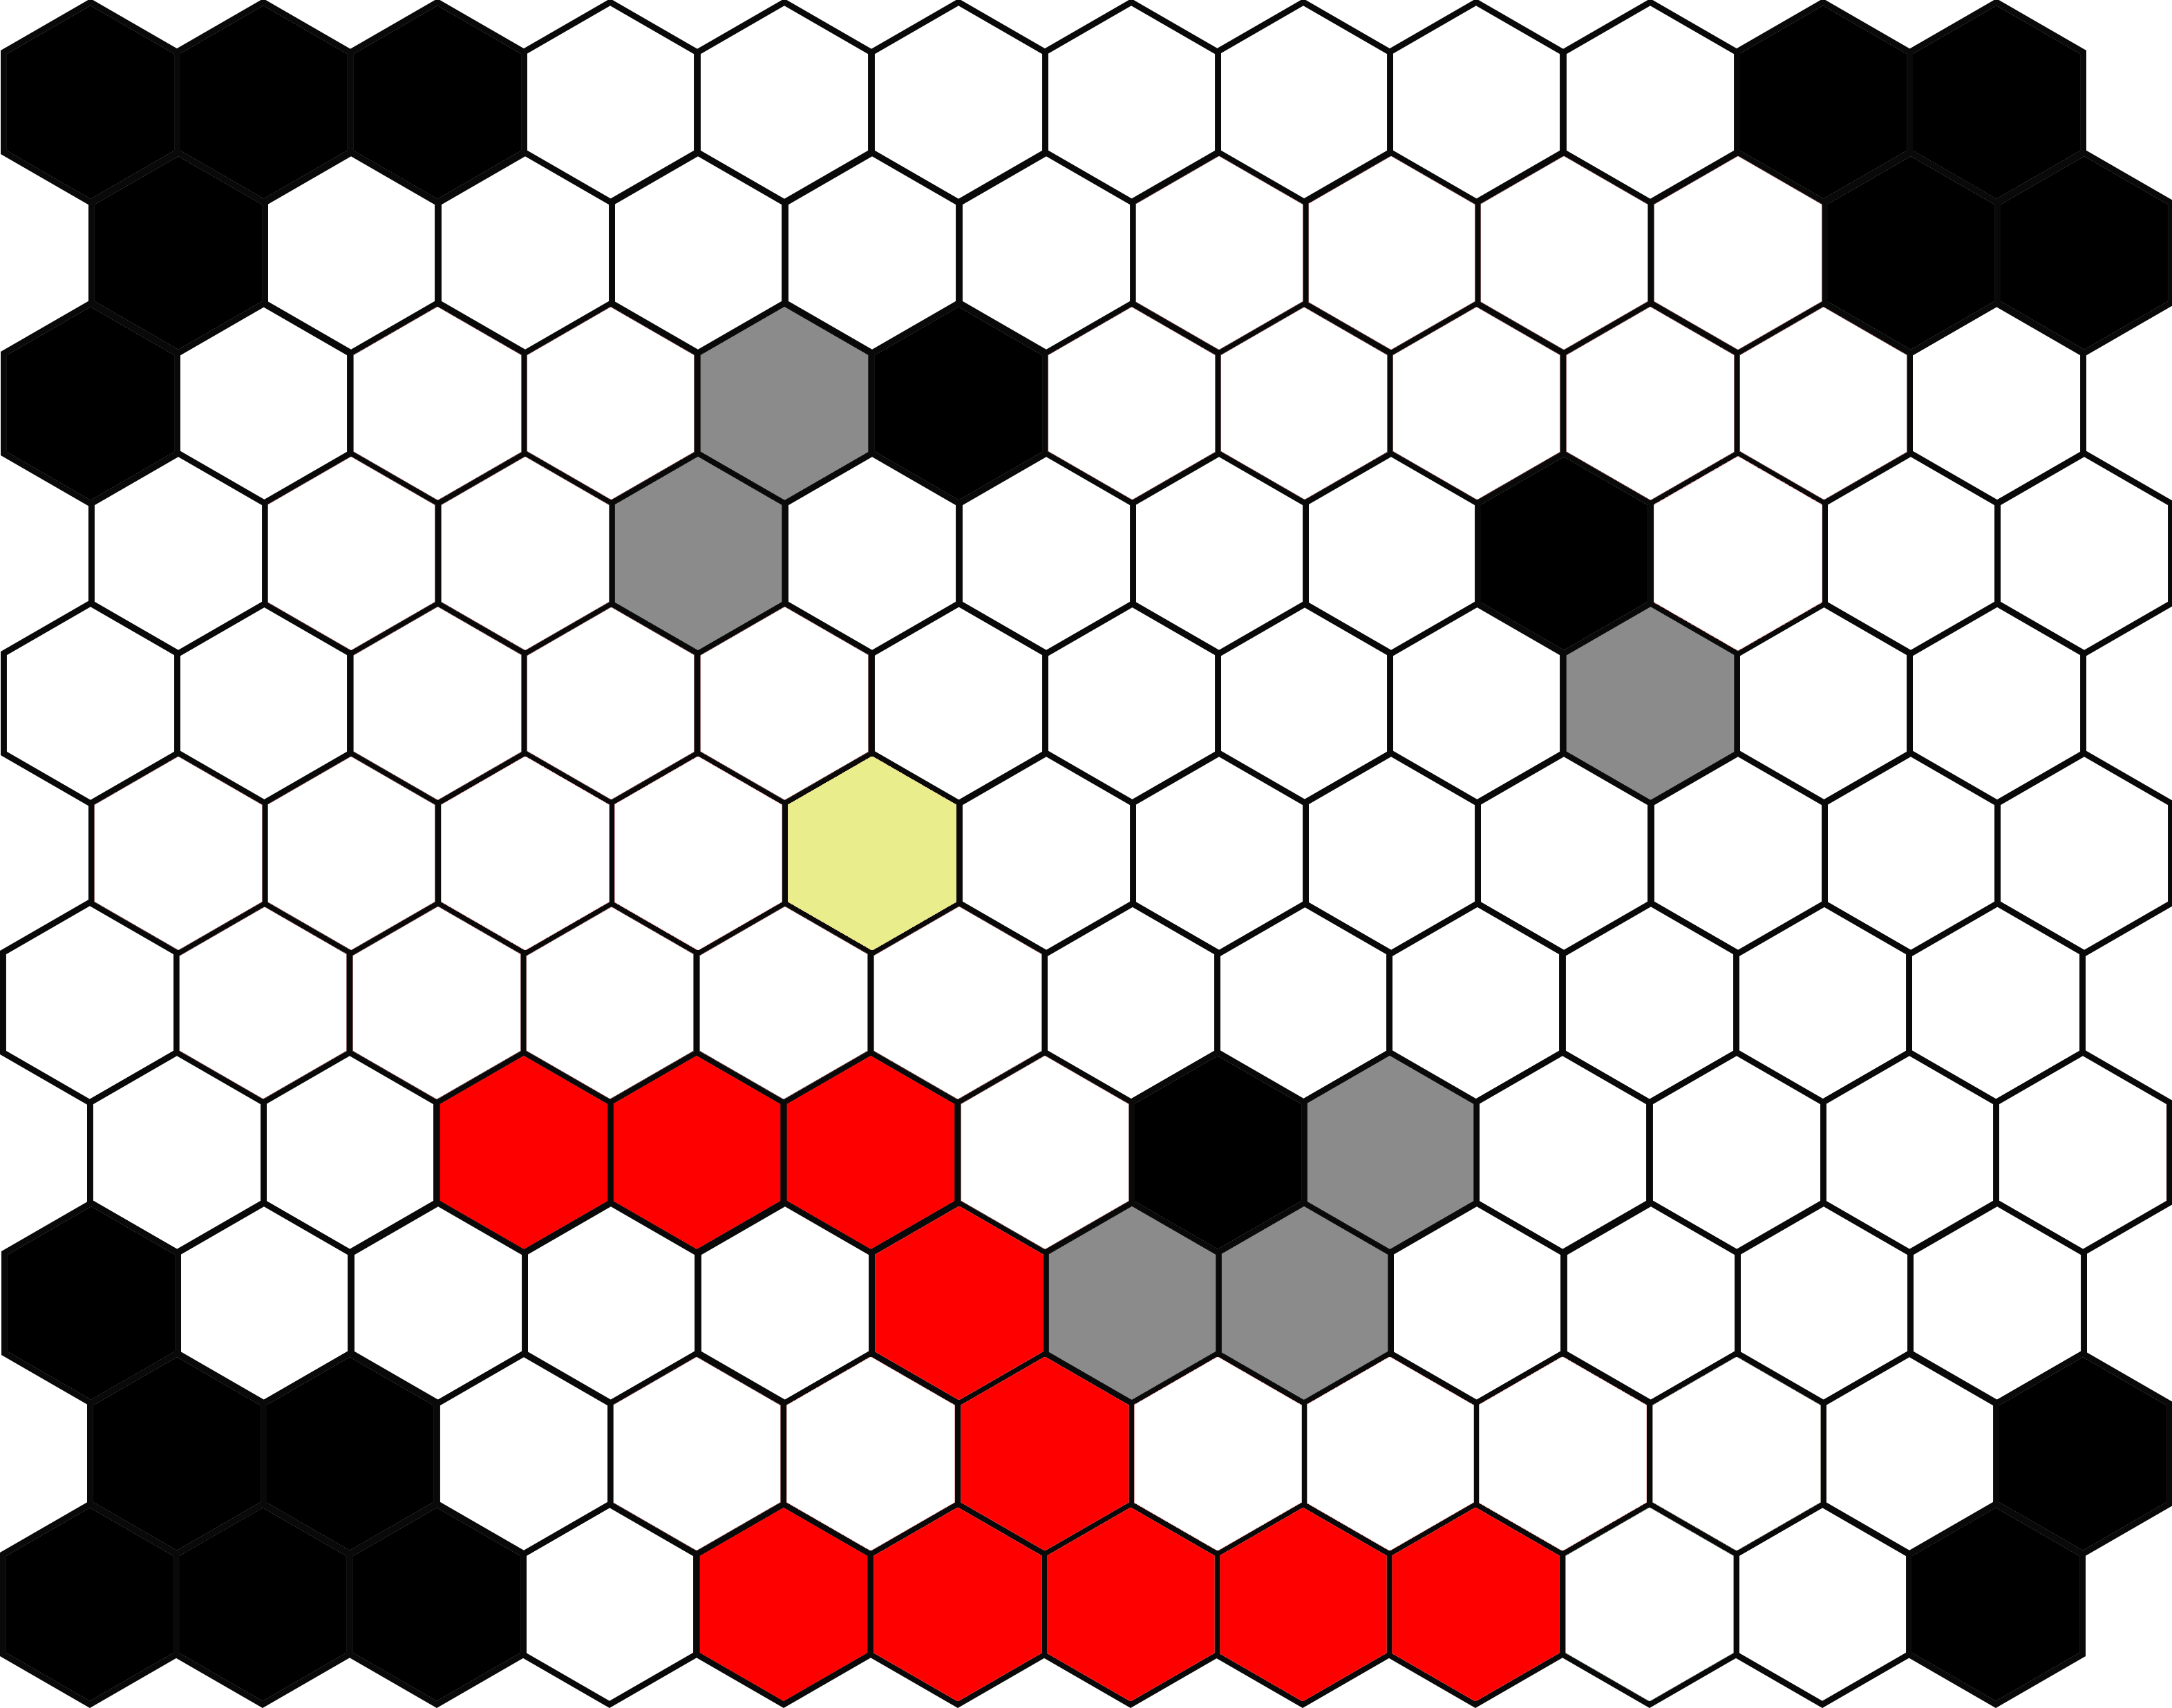
\includegraphics[width = 0.3\textwidth]{./maps/c214e.png}}
\framebox{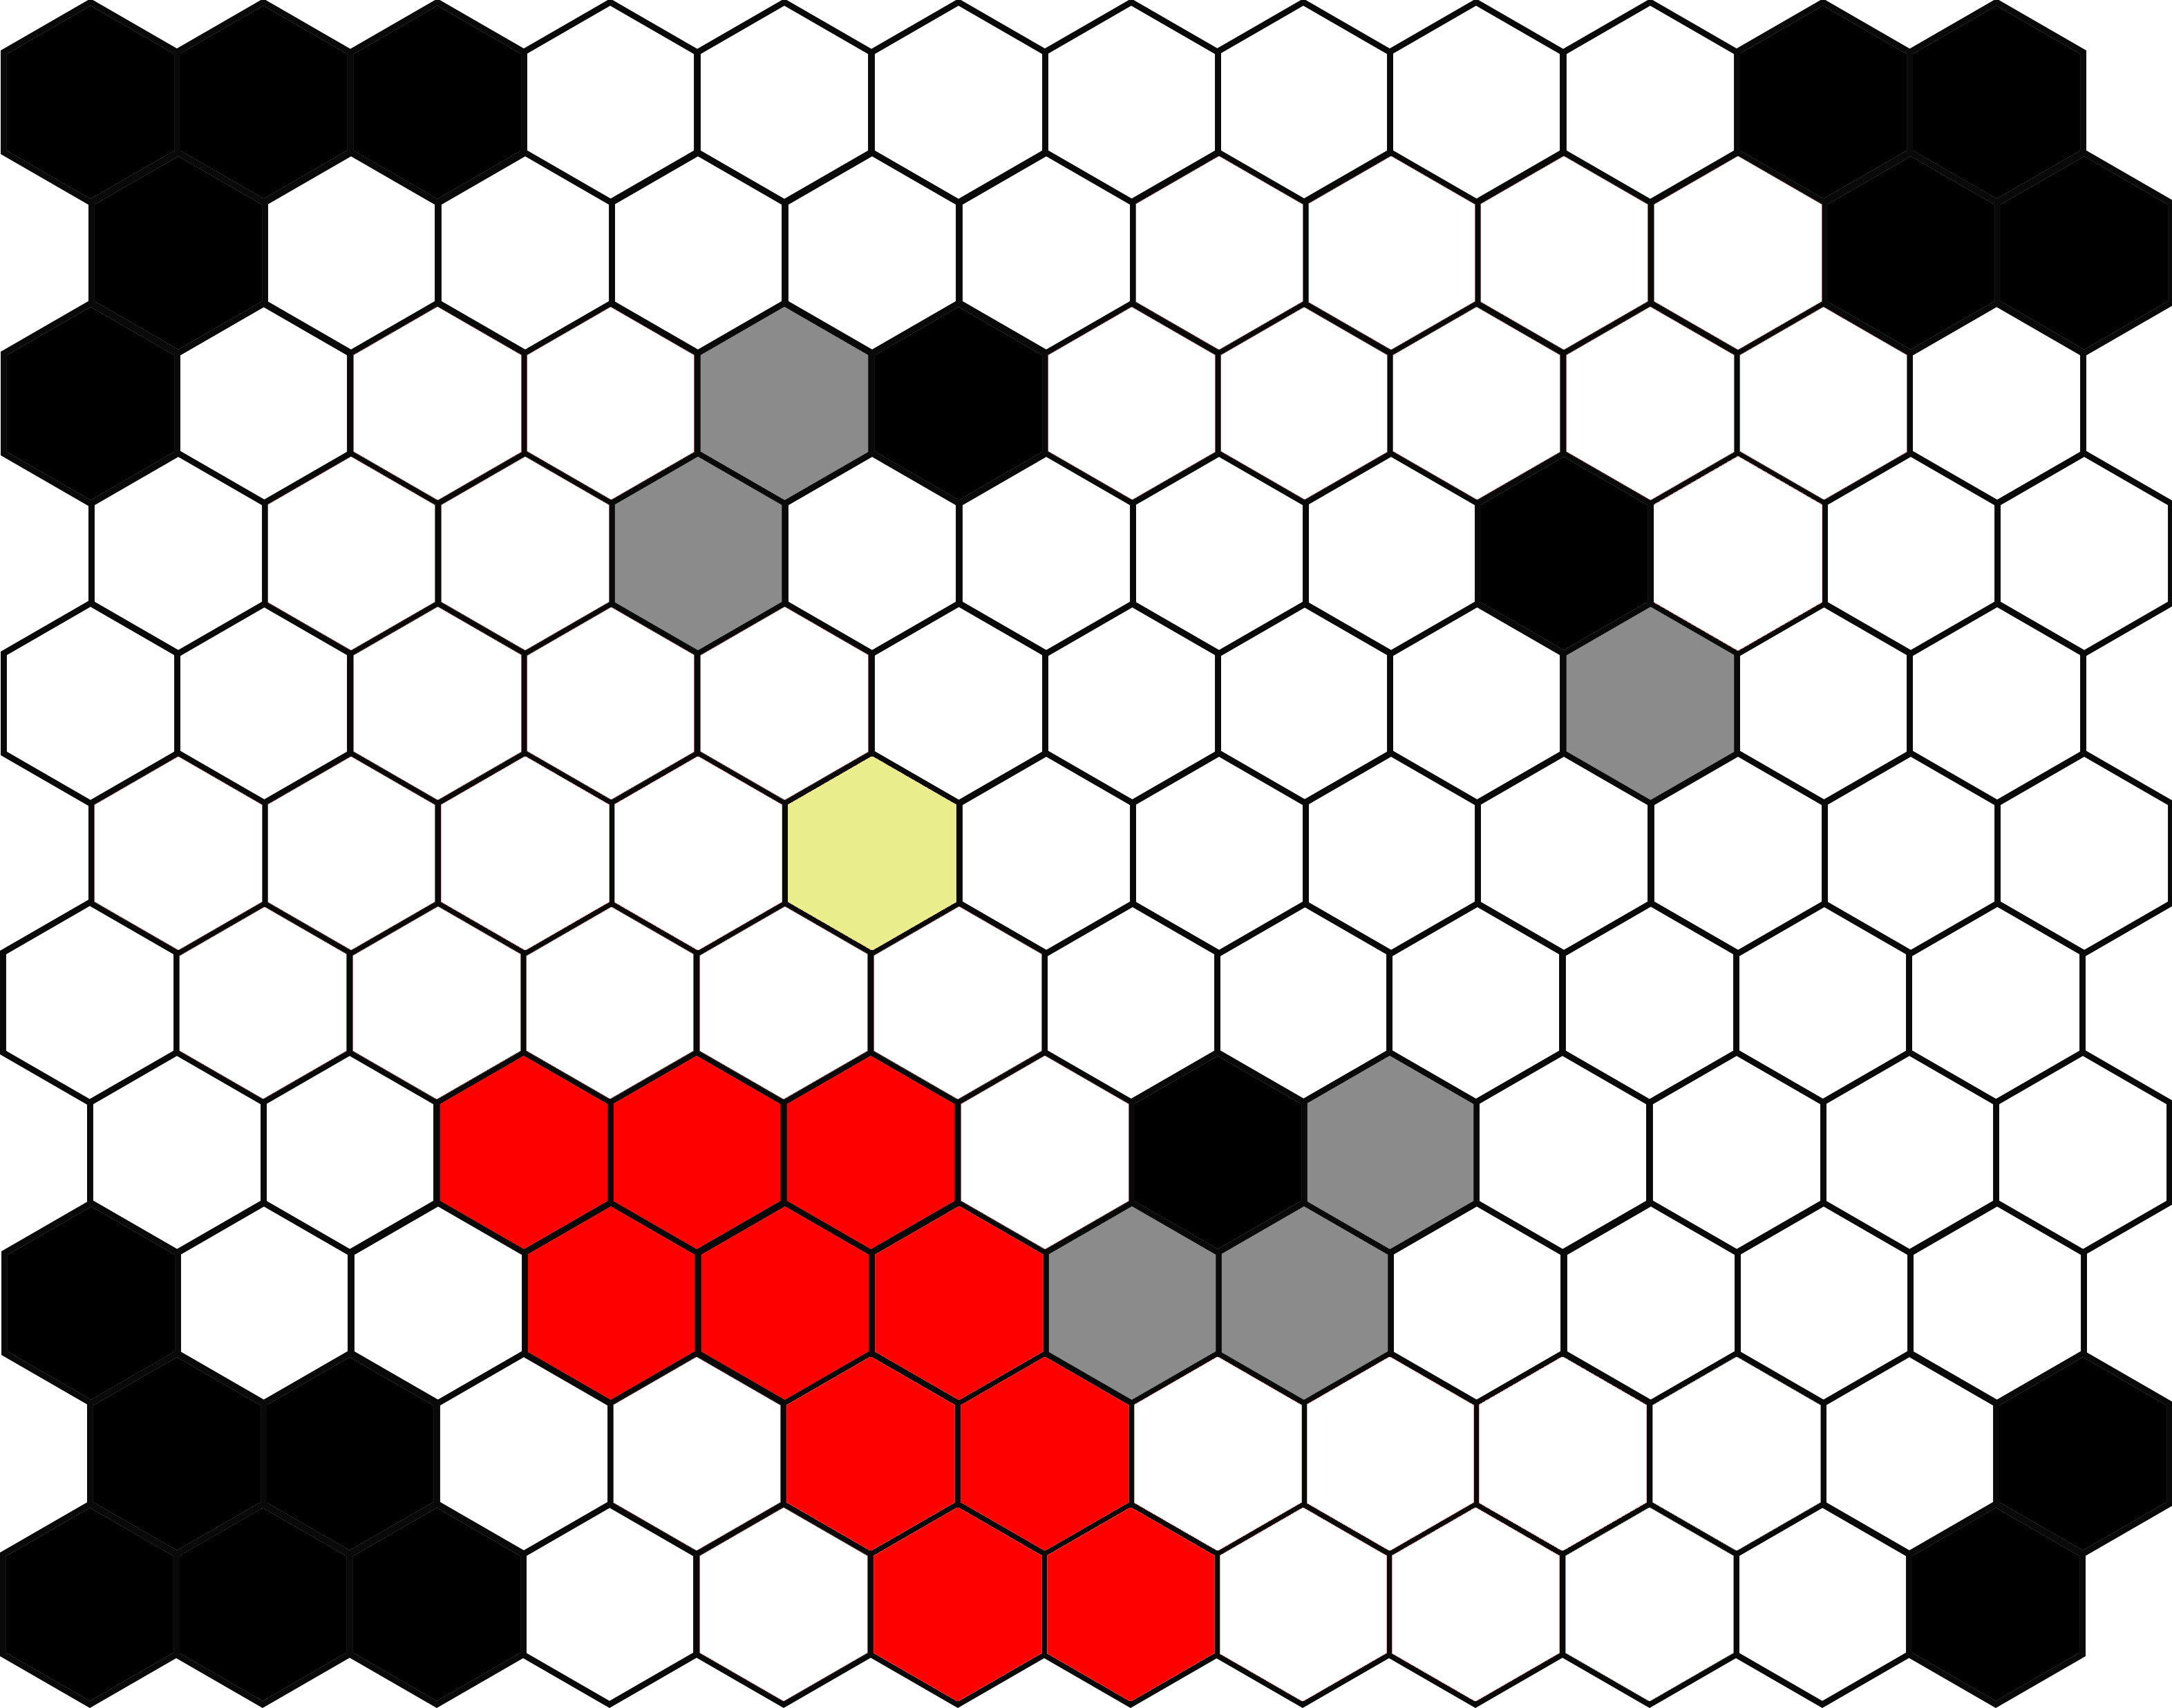
\includegraphics[width = 0.3\textwidth]{./maps/c214f.png}}
\\
\emph{The formation moves sideways via the nearest column if the character stands off to one side.}
\end{center}

\textbf{Attacking} -- After the entire formation has moved, each entity attacks as an individual. Resolve each attack sequentially, starting from entities in the front row. When an encounter roll has multiple attacks, resolve the first attack type for all entities before moving onto the second. Entities in the formation may freely attack past each other.

\pagebreak

\subsection*{Encounter Map}
\begin{center}
\framebox{
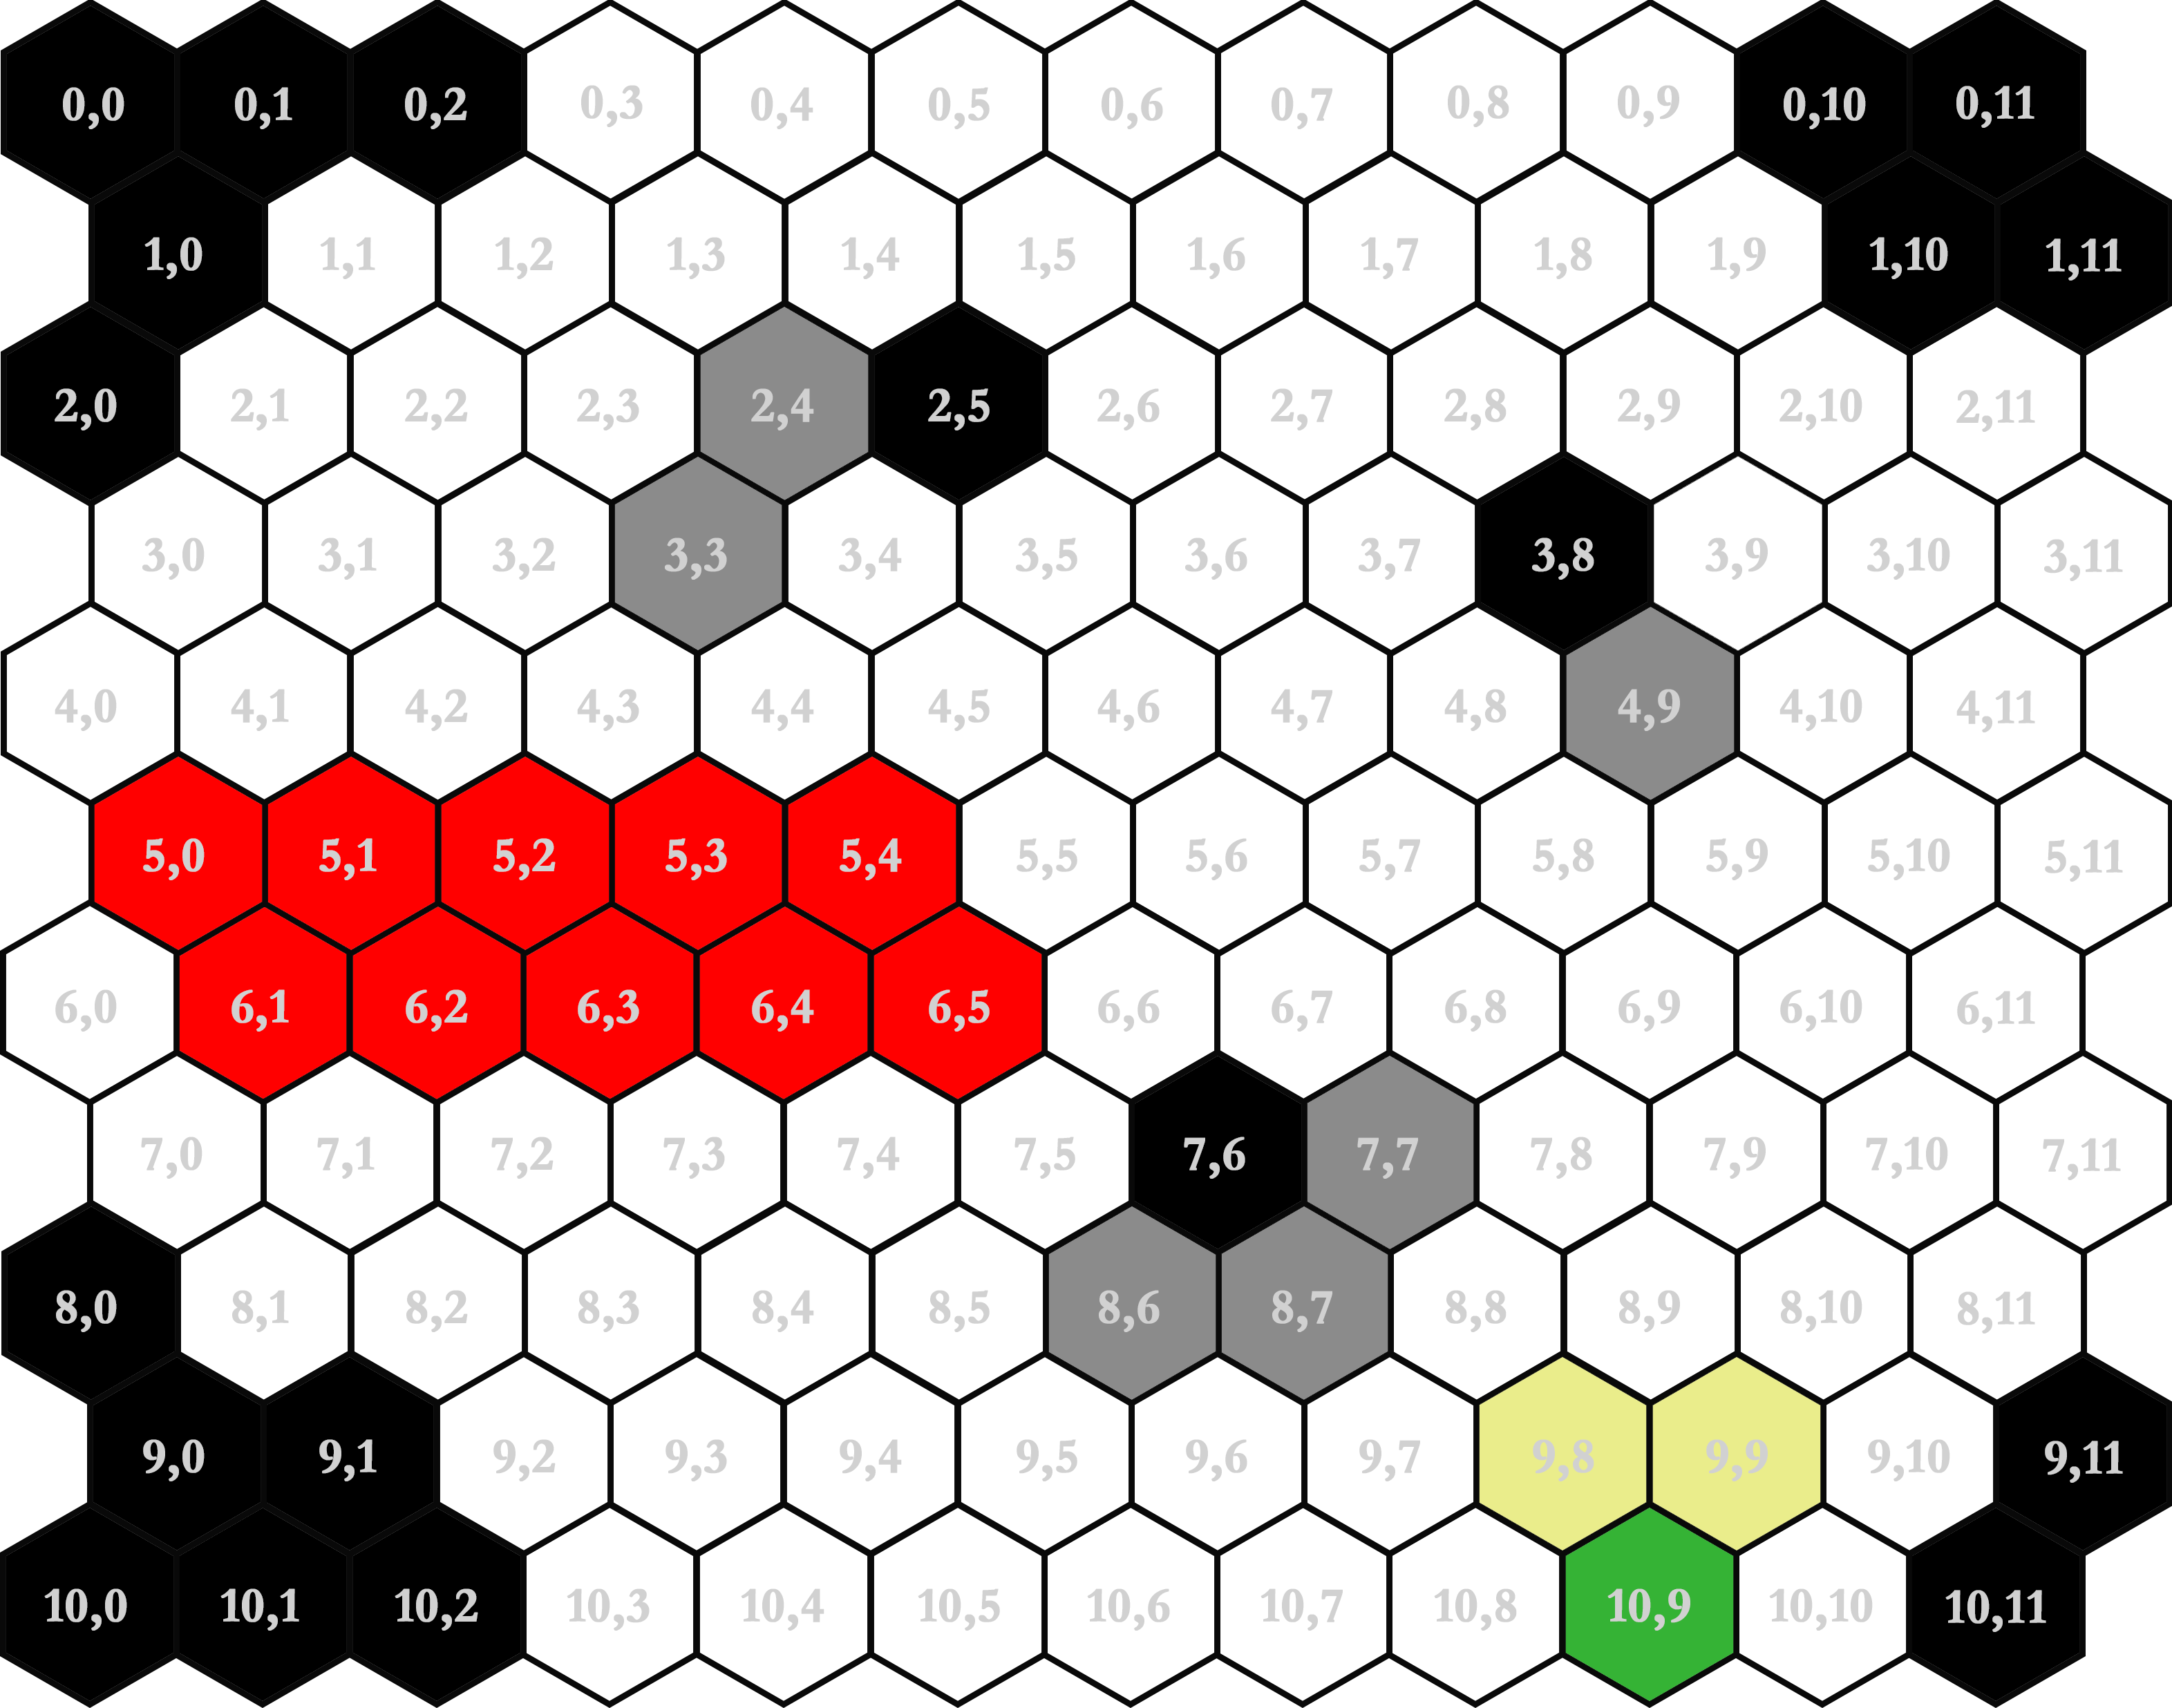
\includegraphics[width = 0.96\textwidth]{./maps/c214.png}
}
\end{center}

\subsection*{Setup Instructions}
\begin{itemize}
\item \textbf{Goldenrod:} Character Start Location. Place the character on either tile.
\item \textbf{Red:} Enemy Start Locations.
\item \textbf{Black:} Full-Cover.
\item \textbf{Gray:} Half-Cover.
\item \textbf{Green:} Escape Tile.
\end{itemize}

\begin{tcolorbox}
\textbf{Hint:} Erase the previous map by holding the page against a wall to avoid getting eraser debris all over your desk.
\end{tcolorbox}

\pagebreak

\subsection*{Victory}
The last of the phalanx falls, his makeshift spear clattering on the flagstone. Despite its crude construction, the weapon was made with ingenuity and great care. Its spearhead, fashioned from the shard of a chamber pot, is secured to the wooden shaft with a rag torn from the man’s own shirt. Looking over the rest of your former comrades, you discover that he didn’t make that alteration alone. The entire phalanx was dressed in a sort of tatterdemalion uniform: their shirts all torn across the chest, displaying the Sign with brazen pride. Everloyal.\\

>> Souls of a Doomed Rebellion (20)\\
\gainx{Warcry}\\
\gain{Makeshift Spear}\\
\gain{Table Shield}\\
\notegain{c214a} The Lost Phalanx is defeated\\
>> \turnto{c215}

\subsection*{Defeat}
A spearhead pierces your flesh, and then another. You stagger backwards, blood pulsing from your wounds like the bungholes of a cask. Your former comrades were damnably well-prepared for this. Even in the throes of madness, they manage to keep up their shieldwall.\\

You have no choice but to flee: scrambling back to fog barrier under a hail of thrown debris. Once beyond the yard, you nurse your wounds and try to think of ways to overcome that phalanx of madmen.\\

>> Immediately resolve the effects of a \emph{short reprieve}\\
>> \turnto{c213}

\subsection*{Retreat}
You flee back through the fog barrier, leaving your former comrades to march their formation aimlessly about the yard. Once beyond the yard, you nurse your wounds and try to think of ways to overcome that phalanx of madmen.\\

>> Immediately resolve the effects of a \emph{short reprieve}\\
>> \turnto{c213}\\

\begin{tcolorbox}
\textbf{Note:} Upon defeat or retreat, this encounter can be repeated as many times as necessary. However, the encounter will begin with The Lost Phalanx at full strength again.
\end{tcolorbox}